\problemname{Triangelskolan}

Kajsa går i Triangelskolan, vars profil är att lägga runda plastbrickor så de bildar liksidiga trianglar. Två exempel visas i figuren. Givet hur många brickor Kajsa har, skriv ett program som beräknar sidlängden för den största triangeln hon kan skapa.
\begin{figure}[ht!]
\centering
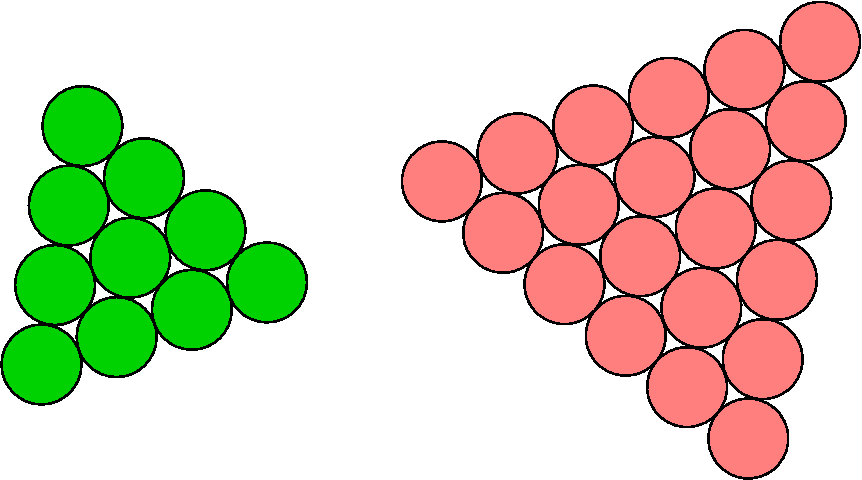
\includegraphics[width=7cm]{triangel.png}
\caption{}
\label{fig1}
\end{figure}

\section*{Indata}
En rad med ett heltal $N$, antalet brickor Kajsa har, där $1\le N \le 1\,000\,000$.
\section*{Utdata}
En rad med ett heltal, sidlängden för den största kompletta triangeln Kajsa kan skapa med högst $N$ brickor.
